\chapter{Production}
\section{Control System}

\section{Power Stage}
\begin{figure}[htbp]
	\centering
	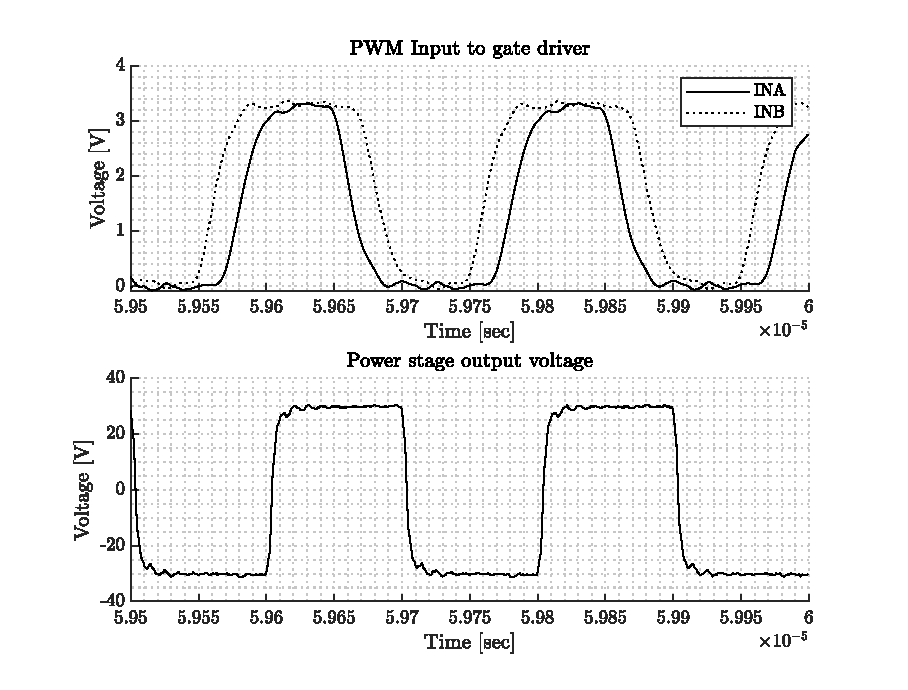
\includegraphics[width=.8\textwidth]{Figures/4_transmitter_pcb_out.eps}
	\caption[Measured input and output of power stage PCB]{Measured input and output of power stage PCB. (Above) Input to gate driver with dead-time (Below) Output of MOSFET half-bridge and the voltage across the load}
	\label{fig:4_transmitter_meas}
\end{figure}
Seen in \cref{fig:4_transmitter_meas} are actual measured inputs and outputs of the power stage. On the input, there are two \qty{5}{\mega\hertz} signals with varying duty cycle to generate the desired dead-time. On the output, we see the rail-to-rail push-pull operation of the \gls{mosfet} half-bridge.
\section{Transmit/Receive Switch}
\section{Preamplifier}

\section{Demodulator}


\section{Pulse-Repetition and Wall Filter}
\section{Digital Signal Processor}
%\begin{figure}[H]
%	\centering
%	\begin{circuitikz}[american voltages]
%		\draw
%		(0,0) to [short, *-] (6,0)
%		to [V, l_=$\mathrm{j}{\omega}_m \underline{\psi}^s_R$] (6,2)
%		to [R, l_=$R_R$] (6,4)
%		to [short, i_=$\underline{i}^s_R$] (5,4)
%		(0,0) to [open, v^>=$\underline{u}^s_s$] (0,4)
%		to [short, *- ,i=$\underline{i}^s_s$] (1,4)
%		to [R, l=$R_s$] (3,4)
%		to [L, l=$L_{\sigma}$] (5,4)
%		to [short, i_=$\underline{i}^s_M$] (5,3)
%		to [L, l_=$L_M$] (5,0);
%	\end{circuitikz}
%	\caption{The nodes short, V, R and L are presented here, but there a lot more}
%	\label{fig:circuitikz}
%\end{figure}

\section{Listings (code)}

\Cref{lst:helloworld} is a nicely formatted block of code. A listing will automatically continue on the next page if it encounters a page break. Many different programming languages can be highlighted. Check the \texttt{listings} package documentation for a list of supported programming languages.

\begin{listing}[htbp]
\begin{mintedc}
#include <stdio.h>
int main()
{
	printf("Hello, World!"); /*printf() outputs the quoted string*/
	if (n == 0 || n == 1){
		return n;
	}
	j = 0;
	for (i = 0; i < n-1; i++){
		if (arr[i] != arr[i+1]){
			arr[j] = arr[i];
			j++;
		}
	}
	arr[j++] = arr[n-1];
	return 0;
}
\end{mintedc}
	\caption{Hello world in C}
	\label{lst:helloworld}
\end{listing}



